\label{JavaAppletCorrectnessKit}
 The main design goals were the following:
 \begin{itemize}
 \item it should provide an easy accessible user interface, that enables average Java programmers to use the tool
 without too much difficulties. This interface is
described section \ref{Industrialisation};
 \item it should provide a high degree of automation, so that most proof obligations can be discharged without user
 interaction. Only in this way, the tool can be effectively used by non-expert users, which is necessary if we want that
 formal methods will ever be used in industry. 
 \item it should provide high correctness assurance: at the moment the prover says that a certain proof obligation
is satisfied, it should be possible to trust this without any reservation. Nevertheless
the tool is not formally developed. It implements, in Java, a weakest precondition calculus that
generates lemmas without user interaction. We cannot prove that those lemmas are necessary and sufficient to
ensure the correctness of the applet but the tool is designed in this way;
 \item it should be independent of any particular prover, so that if the use of a particular prover is
 required (for example by a certification institute) it is relatively easy to adapt the tool accordingly.
\end{itemize}


This section presents the tool architecture and its principles.
\subsubsection{Architecture}
\begin{figure}[tp]
 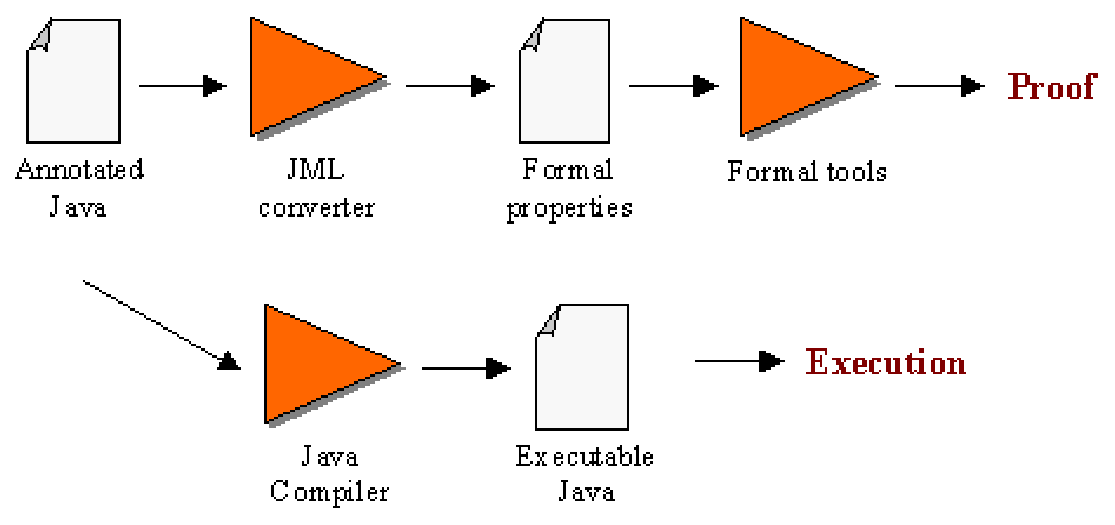
\psfig{file=fm03/image002.eps,width=14cm}
 \caption{\sc \JACK\ architecture}
 \label{JACKarchitecture}
\end{figure}
 Figure \ref{JACKarchitecture} presents an overview of the \JACK\
 architecture.  \JACK\ consists of two parts: a converter (a lemma generator) from
 Java source annotated with JML into JPOL lemmas, and a viewer that
 allows developers to understand the generated
 lemmas.  The viewer is integrated in an IDE and is described more precisely in section
 \ref{Viewer}.  This part focuses on the converter.

 The \JACK\ converter converts a Java class into a JPOL model and allows to
 prove properties. 
 The initial goal was to prove properties on source files written with the Java
 language.  To reach this goal, one has to know how to ``translate'' a
 Java source file in formal lemmas.  

\begin{figure}[p]
 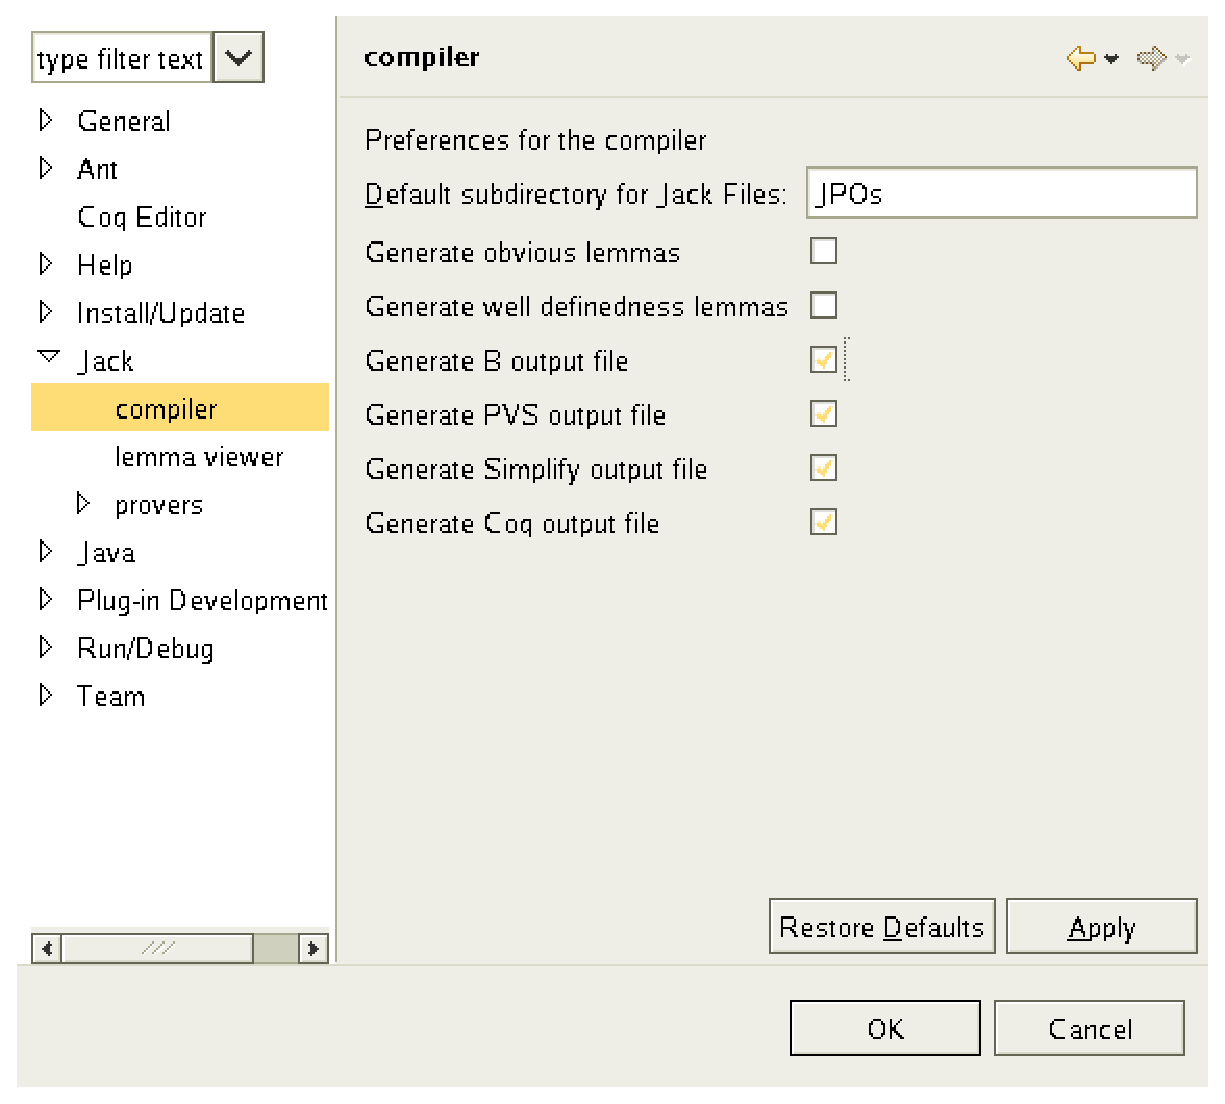
\psfig{file=fm03/preferences-compiler.eps,width=14cm}
 \caption{\sc \JACK\ compiler preferences page}
 \label{JACKcompprefpage}
\end{figure}
 The JML annotations are Java boolean expressions without side
 effects.  Thus, they are easily translated in logical formulas: Java operators are
 translated into functions. For example, shift left (\texttt{<<}) is
 translated into a function associating an integer to a pair of
 integer.  From those translated annotations and the methods code,
 lemmas can be generated automatically.

 From the start, taking into account experiences in lemma generation
 for B machines, we have implemented a Weakest Precondition (WP)
 calculus to automate lemma generation. This involves extending the
 classical Hoare logic to allow the generation of lemmas in the
 context of Java.  The Java statements contain different features like
 control-flow breaks.  So, the classical WP calculus should be
 completed to deal with them.



 Moreover, JML should be lightly upgraded to allow fully automated
 proof obligation generation.  Notably, to automate lemma generation
 for the loops, we have had to extend the JML language with new
 keywords: \texttt{loop\_modifies}.  The \texttt{loop\_modifies}
 keyword allows us to declare the variables modified in the body of
 the loop, as it is done for the methods. During the WP calculus, it
 is necessary to universally quantify the loop invariant with those
 variables, and since they cannot be automatically calculated, one has
 to specify them.

 
 The two main drawbacks of the WP calculus are the loss of information and
 potential exponential explosion.  After lemmas have been generated,
 it is often difficult to understand from which part of the code they
 are derived.  To bypass this issue, program flow information is
 associated to each lemma.  This information is used in the viewer
 to associate an execution path to each lemma. This feature is described in the next section.

 Exponential explosion remains a problem.  Different solutions exist
 to avoid it.  As the WP calculus can be considered as a brute
 force concept, trying to expand all the path of the methods,
 solutions are always based on interaction to reduce this brute force
 by introducing intelligence in the process.

 A simple solution is to require users interaction during lemma
 generation in order to cut unsatisfiable branches.  Rather than introducing
 interaction during generation, another solution is to allow to add
 special annotations in the source code to introduce formulas that are
 taken into account at generation to simplify the lemmas.
 The solution adopted in \JACK\ is to allow to specify blocks. An exponential explosion usually occurs
in a method with many sequenced branched statement ({\tt if, switch}, etc.) Such methods usually perform
different distinct sequenced treatments.
 Figure \ref{Specified_block} presents the skeleton of such a method. Specifying a block (here the second part
of the method) allows to cut proof obligation generation. This corresponds, in fact, to the simulation of a
method call.
\begin{figure}[htp]
{\tt
\begin{tabbing}
 \hspace{3 cm} \=m()\= \ \{ \\
 \> \> \vdots \\
 \> \> if () \{ $\hdots$ \} \\
 \> \> else \{ $\hdots$ \}   \\
 \> \> \vdots                   \\
 \> \> /*\=@ modifies {\it variables}  \\
 \> \> \> @ ensures {\it property} \\
 \> \> \> @\=*/ \{ \\
 \> \> \> \> \vdots \\
 \> \> \> \> if () \{ $\hdots$ \} \\
 \> \> \> \> else \{ $\hdots$ \}   \\
 \> \> \> \> \vdots                   \\
 \> \> \ \} \\
 \> \> \}
\end{tabbing}
}
 \caption{\sc Specified block}
 \label{Specified_block}
\end{figure}

 With those extensions to the JML language, we are able to obtain a fully automated proof obligation generation.
That is the first step to reach user approval. The second one is to propose an access to those lemmas in a
``Java style'', this is described in the next section.
